\begin{solution}{1}
\begin{wrapfigure}{r}{0.3\textwidth}
    \vspace*{-1.5\baselineskip} 
    \centering
    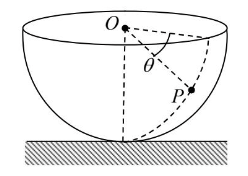
\includegraphics[width=0.9\linewidth]{image/2.png}
\end{wrapfigure}
以滑块和地球为系统，它在整个运动过程中机械能守恒。滑块沿半球面内侧运动时，可将其速度 $v$ 分解成纬线切向（水平方向）分量 $v_{\varphi}$ 及经线切向分量 $v_{\theta}$。设滑块质量为 $m$，在某中间状态时，滑块位于半球面内侧 $P$ 处，$P$ 和球心 $O$ 的连线与水平方向的夹角为 $\theta$。由机械能守恒得
\begin{equation}
\frac{1}{2} m v_{0}^{2} = -mgR \sin \theta + \frac{1}{2} m v_{\varphi}^{2} + \frac{1}{2} m v_{\theta}^{2}
\label{eq:1.s1}
\end{equation}
这里已取球心 $O$ 处为重力势能零点。以过 $O$ 的竖直线为轴。球面对滑块的支持力通过该轴，力矩为零；重力相对于该轴的力矩也为零。所以在整个运动过程中，滑块相对于轴的角动量守恒，故
\begin{equation}
m v_{0} R = m v_{\varphi} R \cos \theta .
\label{eq:2.s1}
\end{equation}
由\eqref{eq:1.s1}式，最大速率应与 $\theta$ 的最大值相对应
\begin{equation}
v_{\max} = v\left(\theta_{\max}\right).
\label{eq:3.s1}
\end{equation}
而由\eqref{eq:2.s1}式，$\theta$ 不可能达到 $\pi/2$。由\eqref{eq:1.s1}和\eqref{eq:2.s1}式，$\theta$ 的最大值应与 $v_{\theta}=0$ 相对应，即
\begin{equation}
v_{\theta}\left(\theta_{\max}\right)=0.
\label{eq:4.s1}
\end{equation}
[\eqref{eq:4.s1}式也可用下述方法得到：由\eqref{eq:1.s1}、\eqref{eq:2.s1}式得
\begin{equation*}
2gR \sin \theta - v_{0}^{2} \tan^{2} \theta = v_{\theta}^{2} \geq 0.
\end{equation*}
若 $\sin \theta \neq 0$，由上式得
\begin{equation*}
\frac{\sin \theta}{\cos^{2} \theta} \leq \frac{2gR}{v_{0}^{2}}.
\end{equation*}
实际上，$\sin\theta=0$ 也满足上式。由上式可知
\begin{equation*}
\frac{\sin \theta_{\max}}{\cos^{2} \theta_{\max}} = \frac{2gR}{v_{0}^{2}}.
\end{equation*}
由\eqref{eq:3.s1}式有
\begin{equation*}
v_{\theta}^{2}\left(\theta_{\max}\right) = 2gR \sin \theta_{\max} - v_{0}^{2} \tan^{2} \theta_{\max} = 0.
\end{equation*}
]
将 $v_{\theta}(\theta_{\max})=0$ 代入\eqref{eq:1.s1}式，并与\eqref{eq:2.s1}式联立，得
\begin{equation}
v_{0}^{2} \sin^{2} \theta_{\max} - 2gR \sin \theta_{\max} \left(1 - \sin^{2} \theta_{\max}\right) = 0.
\label{eq:5.s1}
\end{equation}
以 $\sin \theta_{\max}$ 为未知量，方程\eqref{eq:5.s1}的一个根是 $\sin \theta = 0$，即 $\theta = 0$，这表示初态，其速率为最小值，不是所求的解。于是 $\sin \theta_{\max} \neq 0$。约去 $\sin \theta_{\max}$，方程\eqref{eq:5.s1}变为
\begin{equation}
2gR \sin^{2} \theta_{\max} + v_{0}^{2} \sin \theta_{\max} - 2gR = 0.
\label{eq:6.s1}
\end{equation}
其解为
\begin{equation}
\sin \theta_{\max} = \frac{v_{0}^{2}}{4gR}\left(\sqrt{1+16 \frac{g^{2} R^{2}}{v_{0}^{4}}} - 1\right).
\label{eq:7.s1}
\end{equation}
注意到本题中 $\sin \theta \geq 0$，方程\eqref{eq:6.s1}的另一解不合题意，舍去。将\eqref{eq:7.s1}式代入\eqref{eq:1.s1}式得，当 $\theta = \theta_{\max}$ 时，
\begin{equation}
v_{\varphi}^{2} = \frac{1}{2}\left(v_{0}^{2} + \sqrt{v_{0}^{4} + 16 g^{2} R^{2}}\right),
\label{eq:8.s1}
\end{equation}
考虑到\eqref{eq:4.s1}式有
\begin{equation}
v_{\max} = \sqrt{v_{\varphi}^{2}} = \sqrt{\frac{1}{2}\left(v_{0}^{2} + \sqrt{v_{0}^{4} + 16 g^{2} R^{2}}\right)}.
\label{eq:9.s1}
\end{equation}
\end{solution}